%================================================================================
%       Safety Critical Systems Club - Data Safety Initiative Working Group
%================================================================================
%                       DDDD    SSSS  IIIII  W   W   GGGG
%                       D   D  S        I    W   W  G   
%                       D   D   SSS     I    W W W  G  GG
%                       D   D      S    I    WW WW  G   G
%                       DDDD   SSSS   IIIII  W   W   GGG
%================================================================================
%               Data Safety Guidance Document - LaTeX Source File
%================================================================================
%
% Description:
%   Principles and Process section.
%
%================================================================================
\chapter{Data Safety Management Process (Informative)} \label{bkm:principlesprocess}

\dsiwgSectionQuote{If you can't describe what you are doing as a process, you don't know what you're doing.}{W. Edwards Deming}

\section{Introduction}
To assist organizations with integrating data safety considerations into their existing processes and,
in due course, their safety management system, an outline data safety management process has
been developed.

This is structured around ISO 31000 \cite{citation:iso310002018risk}, and takes into account the data safety assurance principles.
Links between the process objectives and the assurance principles are described in Appendix \ref{bkm:principlesobjectives}. The
adoption of ISO 31000 means that a relatively simple process, which focuses on data-related
aspects, can be presented here and applied by individual organizations.

To simplify the presentation, the process is presented as a series of sequential phases. In practice, a
degree of iteration is likely to be required (e.g., measures adopted to \gls{treat} risks may lead to refined
system design and revised risk analyses). Likewise, it may be appropriate for some parts of the
process to run in parallel (i.e., a subsequent phase may start before a preceding phase has finished).
\begin{figure}[h]
\centering
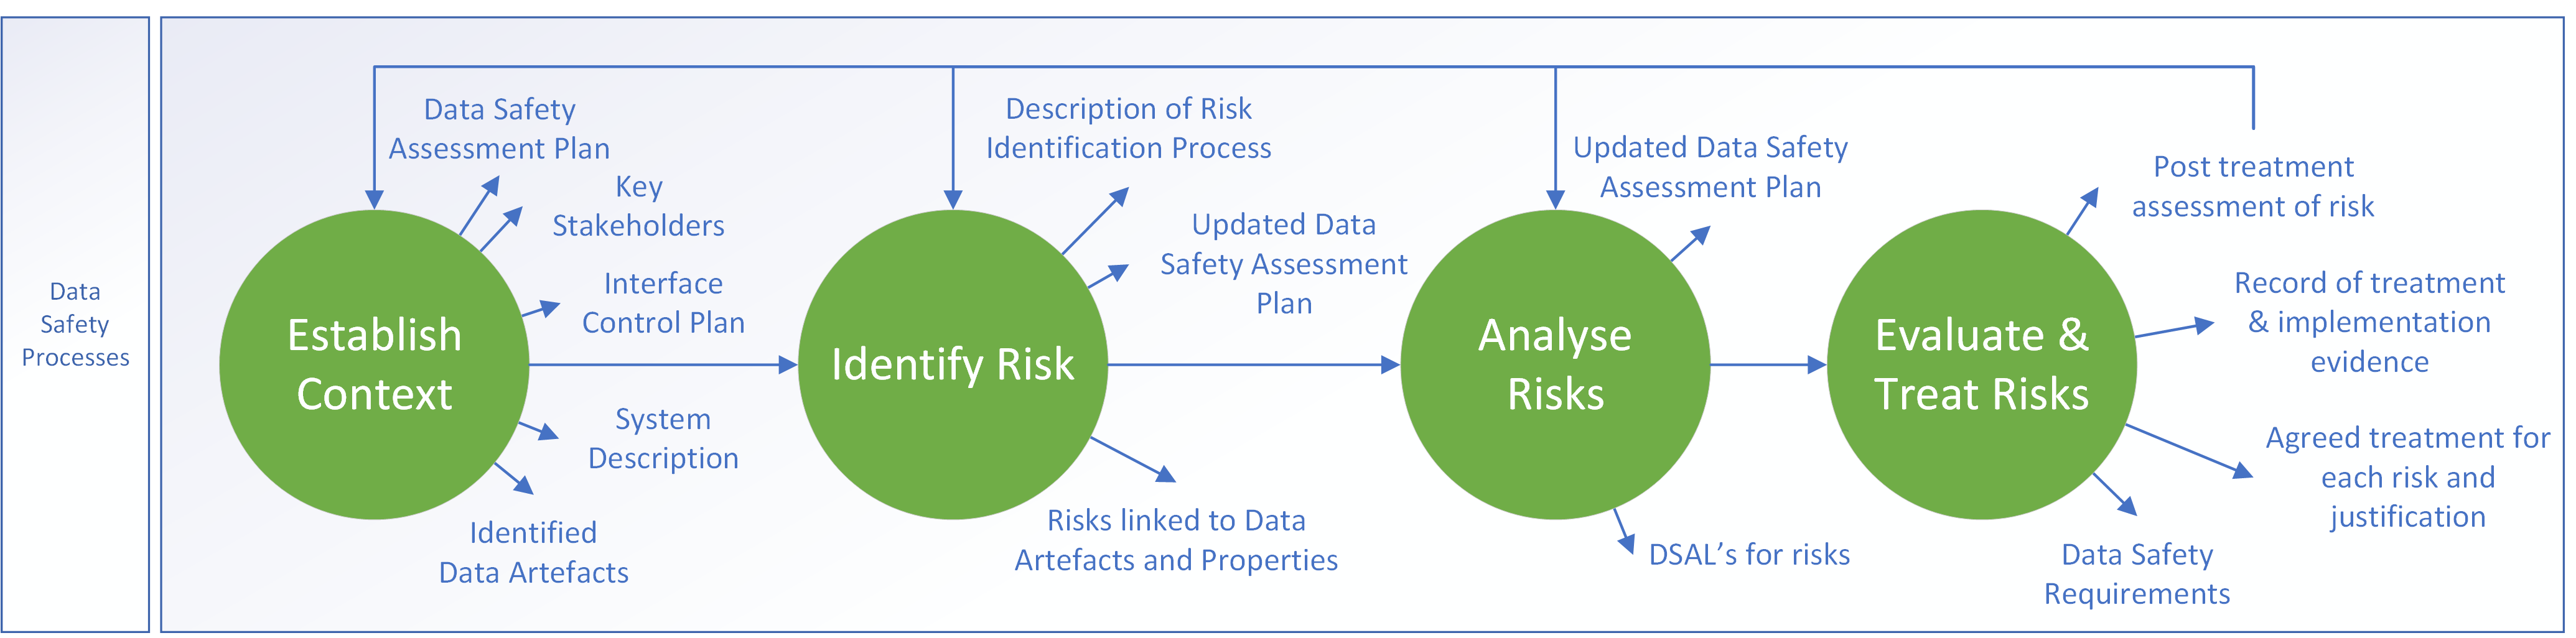
\includegraphics[scale=0.45]{images/process diagram v3 Data Safety Only}
\caption{Process phases}
\label{fig:process_phases}
\end{figure}

The data safety management process occurs over four key steps, each shown as green circles in \autoref{fig:process_phases}, and the specific
objectives and outputs of each step are described in more detail in \autoref{bkm:objectivesoutputs}. The last outcome of the
process is a `post \gls{treatment} risk assessment'. If the risk reduction is not considered adequate, then
the process will iterate again. The whole process is intended to be repeated through the lifecycle of
the system and so will be repeated many times and further iterations will be required when there
are changes to the system or its data.

Although the data safety management process is based on the structure of ISO 31000, there are
some differences between the two. These include:
\begin{itemize}
\item the ISO standard’s ``establish context'' phase is concerned with an organization adopting a
	risk management system; within this guidance document that phase is extended to apply to
	specific projects;
\item the ISO standard considers risk as being synonymous with uncertainty in outcome (i.e.,
	some risks may be beneficial and hence it may be desirable to take actions to increase their
	likelihood); within this guidance document all risks are considered to have adverse effects;
	and
\item the ISO standard separates the ``evaluate risks'' and ``\gls{treat} risks'' activities; within this
	guidance document it has been convenient to combine these into a single phase.
\end{itemize}
ISO 31000 also recommends two activities that run in parallel with risk assessment. These activities
are:
\begin{enumerate}
\item monitor and review the risk assessment process; and 
\item communicate and consult with the
\glspl{stakeholder} about the risk assessment process. 
\end{enumerate}
Aspects such as ``monitor'', ``review'', ``communicate''
and ``consult'' are taken to be part of normal project activities; items such as the \gls{odr} assessment and
the \gls{dsmp} are intended to assist from the perspective of data safety.
\section{Overview}
\begin{figure}[h]
	\centering
	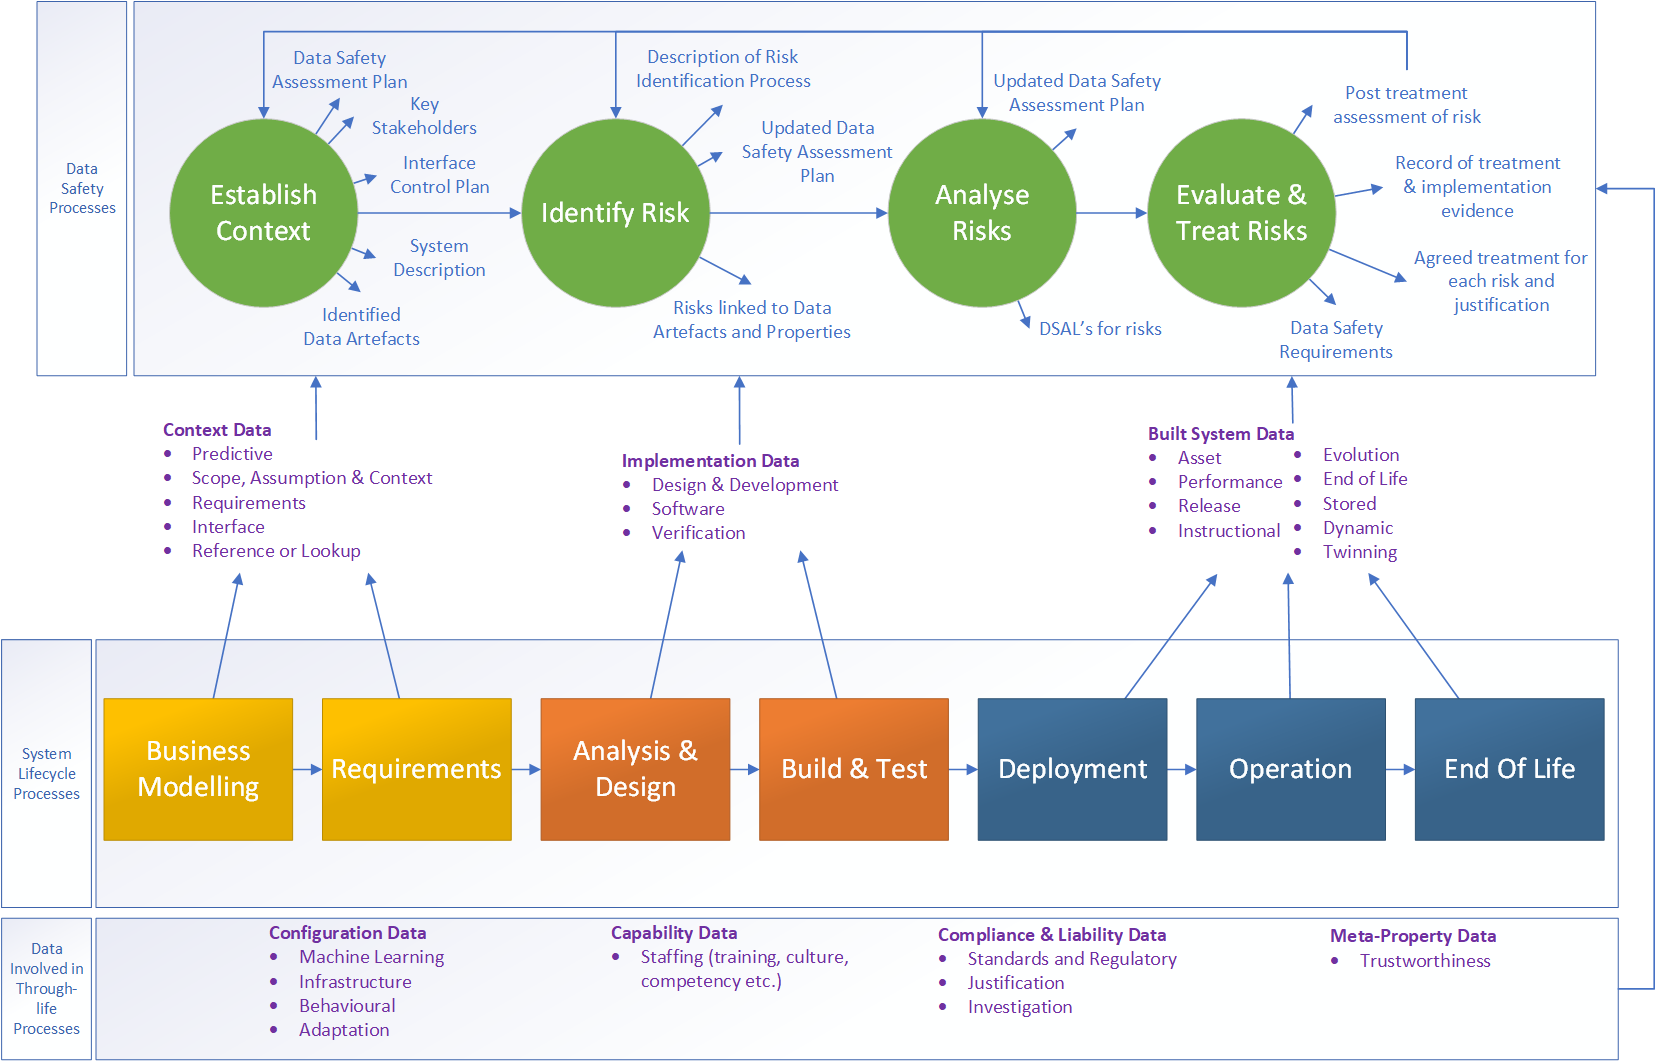
\includegraphics[angle=90,scale=0.6]{images/process_diagram}
	\caption{Simplified process overview}
	\label{fig:process}
\end{figure}
\autoref{fig:process} provides an overview of how the of the \gls{dsmp}
integrates with a typical system lifecycle. 
The system lifecycle is illustrated in the diagram as a simple
model of sequential phases, with each phase shown as a coloured rectangle (phases are coloured for
clarity; colour otherwise imbues no other particular meaning. Lifecycles may of course be more
iterative, involve parallel streams etc., but this simple model suffices to illustrate the concepts).
Further examples of system lifecycles are given in Appendix I.

In practice, the main \gls{safety assessment} activities will
occur as part of the normal safety assessment process lifecycles, so, for example, when considering risks arising
from failures of the software and hardware of a system, loss of properties of data should also be
considered.

Data, however, pervades all aspects of a systems lifecycle so the \gls{safety assessment}
process can occur throughout the system lifecycle depending on the type of data that is being
assessed. Some \glspl{item data} such as context, implementation and built system data are relevant for
specific process phases of the lifecycle, while others such as configuration, capability, compliance and
liability data apply throughout the entire lifecycle. The meta-property data of trustworthiness
covers data that is used to inform on the overall trustworthiness of the system. The specific data
categories are covered in more detail in \autoref{bkm:datacategories} and \autoref{bkm:categories}.

The types of data that are of concern for each process step including those that apply to all steps are
shown and these feed into the data safety assessment process.
